\chapter{Implementation}
\label{ch:implementation}

This chapter will describe the proposed solution for implementing a smart contract in this thesis reflecting the requirements outlined in the previous chapter. This will include explaining: 1) The chosen data structure for the smart contract; 2) The necessary functions for the smart contract; 3) Installing the Web3 framework which is used to connect the smart contract to the Blinky application and 4) The solutions to handle potential error during the lifetime of the smart contract.

\section{Smart contract data structure}
\label{section:DataStructure}

In order to write and read Cost-Split data (as described in Section \ref{section:requirements}), the data structure of the smart contract will need to be defined. Figure \ref{fig:smartcontractdatastructure} provides a visualized data structure plan. Since each Cost-Split should have its own space to store its event data, one such option for organizing Cost-Splits could be using a \texttt{mapping} \citep{SolidityMapping}. Each Cost-Split will be identified from the key obtained from the Blinky API server, as described in Section \ref{blinkyAPI}. This will make Cost-Split fetching as quick and efficient because to find an element in a \texttt{mapping} data structure knowing the key (in this case, the Cost-Split's identifier) only need an asymtotic performance of $\Theta(1)$. 

Each event of a Cost-Split will need to carry a description, timestamp and the identifier of the person who initiates the event. Hence, \texttt{struct} data type is the only candidate for defining the data structure of a Cost-Split event. This \texttt{struct} will contain a \texttt{string} type for the description and another \texttt{string} type for the time stamp in the ISO 8601 format \citep{ISOFormat} (such as \texttt{2018-11-12T19:26:47.858Z}) since this format is compatible with various programming languages. The \texttt{struct} will also contain an \texttt{uint} field for storing the user's identifier from Blinky API Service. After this passage, the \texttt{struct} will be refered to as the \texttt{CostSplitEvent} type.
\label{DataStructure}

\begin{figure}[h!]
    \centering
    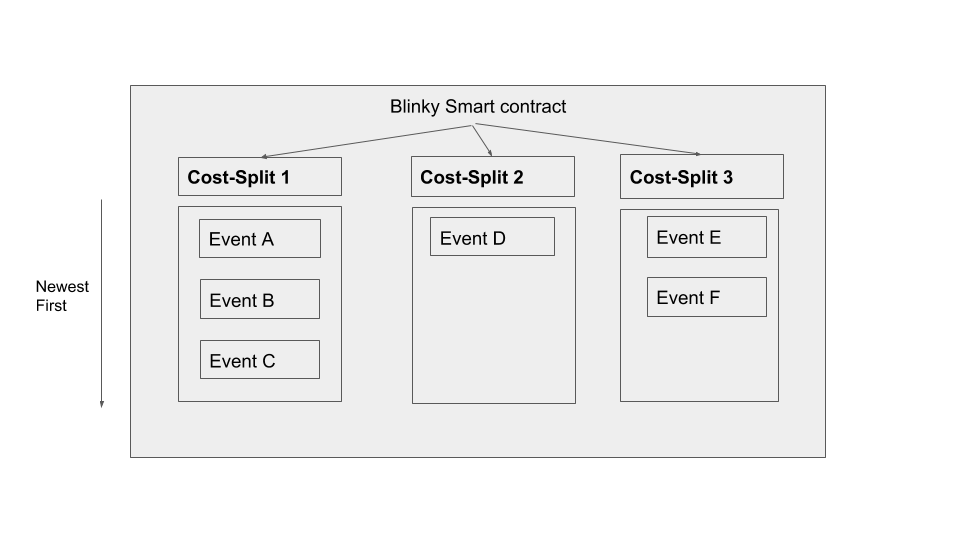
\includegraphics[width=\linewidth]{BlinkyCostSplitSmartContractDataStructure.png}
    \caption{Blinky's Cost-Split Smart contract data structure \citep{RefWorks:doc:MasteringBlockchain}}
    \label{fig:smartcontractdatastructure}
\end{figure}


Furthermore, after being able to access the data of a Cost-Split using its key, each event should be sorted chronologically. Therefore, the smart contract will need to store the Cost-Split data as an \texttt{Array} of \texttt{CostSplitEvent}. Since each event will be recorded chronically by nature, no sorting operation is necessary on the array.

\section{Smart contract functions}
\label{section:SmartContractFunctions}

Since the smart contract will need to be able to create a new data slot for a Cost-Split, a function is needed, which can be named as \texttt{createCostSplit}. This function should accept the identifier of the Cost-Split as a parameter and should return a \texttt{boolean} type to indicate if the creation is successful or not, either \texttt{true} or \texttt{false}.

After a Cost-Split is created, users will then began to interact with it in the Blinky Application, which will incur events. Therefore, a new function is needed to start to add new events into a Cost-Split. This function can be called \texttt{appendEvent}. In order to identify the Cost-Split and to write the necessary data field of the event as specified in Section \ref{DataStructure}, the function will need to receive the identifier of the Cost-Split, the identifier of the Blinky user who initialized the event, the event's time stamp and the event description as the parameter. This function should also denote if the action completes successfully or not so it should return a \texttt{boolean} type like \texttt{createCostSplit}. Figure \ref{lst:appendEventFunction} outlined the function's signature as described above for the purpose of demonstration.

\begin{lstlisting}[float,caption={Skeleton implementation of function \texttt{appendEvent}.},label={lst:appendEventFunction},language=Solidity]

contract BlinkyCostSplit {
 ...
 function appendEvent(
    uint costSplitId,
    uint userId,
    string timestamp,
    string eventDescription) returns (bool) {
   // The function's implementation
   return true;
 }
 ...
}

\end{lstlisting}

In a normal data management software, there should be functions for creating, reading, updating and deleting data. However, in this particular smart contract, data should not be updated or deleted, since the aim of the smart contract is to embrace the transparency, which means data should be as it is from the moment of being created. Users' will to update or delete Cost-Split's events should, therefore, be added to the event list as a new event with the description of what is user's will.

\section{Web3 Framework}

After defining the data structure (mentioned in Section \ref{section:DataStructure}) and the functions needed for the smart contract (as mentioned in \ref{section:SmartContractFunctions} ), knowing a tool for communicating with the smart contract from the outside Internet is necessary, and such an option for it called the Web3 Framework exists. The advantage of this framework that it is written in the Javascript programming language, which is also used in the React Native framework in the Blinky mobile application. Hence, this enables fast and easy integration of the framework to both the web page and the mobile application of Blinky. In order to install and configure the Web3 Framework, the following steps are required:

\begin{itemize}
    \item React Native projects's dependencies can be managed using the \texttt{npm} package manager. Therefore, the content of the Web3 Framework can be downloaded from \texttt{npm}
    \item Choose a suitable Framework version that is compatible with React Native. There are two newest versions: 1.0 and 0.20.x during this time of writing this thesis. Version 1.0's content is generated dynamically, which is not compatible with React Native due to the nature of a mobile application (the code inside the app will be static after being built). Therefore, version 0.22.x is chosen to be installed.
    \item Pony-fill some APIs of Javascript that React Native does not support, such as the \texttt{crypto} API to perform encryption and hashing. Those can be solved by installing package \texttt{node-libs-react-native}
\end{itemize}

There are also community composed tutorials, one of which can be found on the web site link: \citep{InstallWeb3}
After following the above mentioned steps and conducting other smaller tweaks as presented in the link above, The web3 framwework can be invoked in React Native as an example in Program \ref{lst:callweb3}

\begin{lstlisting}[float,caption={Calling Web3 functions and making transactions on the Ethereum blockchain \citep{SolidityDocumentation}.},label={lst:callweb3},language=Javascript]

const web3 = new Web3(Web3.givenProvider);
const contractAddress = "0x1a5c29c94D03C4c8f7414564CBD57295d61e898f";
const contractAbi = [
	{
		"constant": false,
		"inputs": [
			{
				"name": "x",
				"type": "uint256"
			}
		],
		"name": "set",
		"outputs": [],
		"payable": false,
		"stateMutability": "nonpayable",
		"type": "function"
	},
	{
		"constant": true,
		"inputs": [],
		"name": "get",
		"outputs": [
			{
				"name": "",
				"type": "uint256"
			}
		],
		"payable": false,
		"stateMutability": "view",
		"type": "function"
	}
];
const myContract = web3.eth.contract(contractAbi);
myContract.methods.myMethod("set")
  .send({from: '0xde0B295669a9FD93d5F28D9Ec85E40f4cb697BAe'})
  .then(function(receipt){})
  .catch(function (error) {});

\end{lstlisting}

In Program \ref{lst:callweb3}, first an instance of the web3 framework is instantiated, with the default provider bundled within the framework. Then the contract address contract address and it's Application Binary Interface (ABI) is specified in line 3, 4and then passed to the initialization function that creates an instance of \texttt{web3.eth.contract} in line 34, which represents an Ethereum smart contract. After that, the program can start calling the functions on the smart contract by calling function \texttt{methods.myMethod} on the contract instance (as presented in line 36 to 38.

\section{Error handling}

Error handling is one of the most important aspects to consider when developing a software product, to ensure that the software works as expected and maintains a high-quality user experience. In this case of implementing the smart contract for storing Cost-Split event, there are cases which may confuse the smart contract and therefore handling the errors while developing the smart contract is a vital step.

Errors that can happen are when the smart contract tries to add an event to a non-existing Cost-Split, or in other words, the function \texttt{appendEvent} is given an invalid Cost-Split identifier. In solidity, this function invocation will result in throwing an \texttt{Exception}, all the changes to smart contract during that function call will be reverted and the failure will be notified to the caller (in this case, the Blinky Application). However, this kind of error without being handled will degrade user experience since they may not be aware of how the Blinky Application handles the event sending. This thesis will propose a way to handle this error:

 The smart contract's function will use \texttt{require} function as a way to verify the validity of the data (in this case, checking the Cost-Split's identifier if it exists in the smart contract's state). If the assertion does not satisfy, the function will throw an early \texttt{Exception} to tell that the identifier is not valid. The Blinky Application can catch this Exception and display an appropiate dialog to notify user. An example of this error handling is presented in Program \ref{lst:assertValidateInput}. From the Program, it is noted that in Solidity, the default value for a variable is 0 if it has not been set to any value yet. Hence, it is possible to check for the existence of a Cost-Split in the smart contract's state by trying to access its value inside \texttt{mapping costSplitMap}, then compare it to 0. The error message "Cost Split does not exist in the smart contract" will be thrown if the assertion fails.

\begin{lstlisting}[float,caption={Using \texttt{require} function to validate input data},label={lst:assertValidateInput},language=Solidity]
contract BlinkyCostSplit {
 
 struct CostSplitEvent {
    uint userId;
    string description;
    string timestamp
 }
 
 mapping(uint => CostSplitEvent) costSplitMap;
 
 function appendEvent(
    uint costSplitId,
    uint userId,
    string timestamp,
    string eventDescription) returns (bool) {
   // The function's implementation
    require(
        costSplitMap[costSplitId] != 0,
        "Cost Split does not exist in the smart contract"
    );
   // ... Remaining implementation for this function
   return true;
 }
 ...
}
\end{lstlisting}